\documentclass[titlepage, a4paper, openbib, 10pt]{article}

%#####################################
%Usepackages en installingen
\usepackage[top=1in, bottom=1in, left=1in, right=1in]{geometry}
\usepackage[pdftex]{graphicx}
\usepackage{fancyhdr}
\usepackage{sectionbox}
\usepackage[dutch]{babel}
\usepackage{chngcntr}
\usepackage{cite}
\usepackage{url}
\usepackage{makeidx}
\usepackage{paralist}
\usepackage{enumitem}
\usepackage{tocloft}
\usepackage{listliketab}	
\usepackage[table]{xcolor}
\usepackage{tabularx}
\usepackage{epsfig}
\usepackage{pdflscape}
\usepackage{pdfpages}
\usepackage{float}
\usepackage{multirow} 
\usepackage{rotating}
\usepackage[utf8]{inputenc}
\usepackage{color}
\usepackage{fp}
\usepackage{draftwatermark}
\SetWatermarkText{\textsc{Concept}}
\SetWatermarkScale{5}
\newcommand{\red}[1]{
\textcolor{red}{#1}
}
\usepackage{listings}
\lstset{language=C,
basicstyle=\ttfamily\footnotesize,
frame=shadowbox,
mathescape=true,
showstringspaces=false,
showspaces=false,
breaklines=true}


%\usepackage{showframe} %tmp
%#####################################
%Nieuwe commando's
\newcommand{\HRule}{\rule{\linewidth}{1pt}}
\newcommand{\organisatie}{\uppercase{Hogeschool Rotterdam / CMI}}
\newcommand{\modulenaam}{Development 2}
\newcommand{\modulecode}{\uppercase{INFDEV02-2}}
\newcommand{\stdPunten}{4}
\renewcommand{\author}{Dr. Giuseppe Maggiore, Tony Busker}

\definecolor{lichtGrijs}{RGB}{169,169,169}



%#####################################
%Index en styling
\setlength{\cftbeforesecskip}{10pt}
\setlength\parindent{0pt}
\makeindex
\graphicspath{{../Img/}}
\counterwithin{figure}{subsection}
\pagestyle{fancy}
\setcounter{secnumdepth}{5}
\setcounter{tocdepth}{5}

%#####################################
%     Alles voor header/footer
\fancyhf[HL]{\nouppercase{\textit{\leftmark}}}
\setlength{\headheight}{36pt}
\lhead{\uppercase{\footnotesize Course description}}
\chead{\footnotesize \organisatie}
\rhead{
\includegraphics[width=0.09\textwidth]{logo}}

\lfoot{\scriptsize \modulenaam}
\cfoot{\scriptsize \today}
\rfoot{\small \thepage}

\renewcommand{\headrulewidth}{0.4pt}
\renewcommand{\footrulewidth}{0.4pt}
%#####################################

\begin{document}

%#####################################
%Titlepage
\begin{titlepage}
\thispagestyle{fancy}
\ 
\vspace{5cm}

\begin{center}

	
	\Large \textbf \organisatie
	
	\vspace{1.5cm}
	
	\HRule \\[0.4cm]
	
	\Huge \textbf \modulenaam
	
	\vspace{1.7cm}
	
	\Large \textbf  \modulecode
	
	\vspace{0.4cm}
	
	\HRule \\[1.5cm]
\end{center}
\vfill

% Author and supervisor
\begin{tabular}{l l}
	Number of study points:  & \stdPunten{} ects\\
	Course owners: & \author\\
\end{tabular}

\end{titlepage}

%####### Contentpagina ########
%\renewcommand{\baselinestretch}{1.5}\normalsize
%\tableofcontents
%\newpage
%\listoffigures
%\newpage
%\listoftables
%\newpage

%########### Inhoud ###########

\shadowsectionbox
\section*{Modulebeschrijving}
\begin{tabularx}{\textwidth}{|>{\columncolor{lichtGrijs}} p{.26\textwidth}|X|}
	\hline
	\textbf{Module name:} & \modulenaam\\
	\hline
	\textbf{Module code: }& \modulecode\\
	\hline
	\textbf{Study points \newline and hours of effort:} & This module gives \stdPunten{}  ects, in correspondence with \FPeval{\result}{clip(\stdPunten*28)}\result{} hours:
	\begin{itemize}
		\item 3 x 6 hours frontal lecture
		\item 3 x 6 hours practicum
		\item the rest is self-study
	\end{itemize} \\
	\hline
	\textbf{Examination:} & Written examination and practicums (with oral check) \\
	\hline
	\textbf{Course structure:} & Lectures, self-study, and practicums \\
	\hline
	\textbf{Prerequisite knowledge:} & Basic imperative control structures and datatypes, as per INFDEV02-2. \\
	\hline
	\textbf{Learning tools:}  &
		\begin{itemize}
			\item Book: Think Python; author A. B. Downey (\url{http://www.greenteapress.com/thinkpython/})
			\item Book: The Coder’s Apprentice; author Pieter Spronck (\url{http://www.spronck.net/pythonbook/pythonbook.pdf})
			\item Presentations (in pdf): found on N@tschool and on the GitHub repository \url{https://github.com/hogeschool/INFDEV02-2}
			\item Assignments, to be done at home and during practical lectures (pdf): found on N@tschool and on the GitHub repository \url{https://github.com/hogeschool/INFDEV02-2}
		\end{itemize} \\
	\hline
	\textbf{Connected to \newline competences:} &
	\begin{center}
		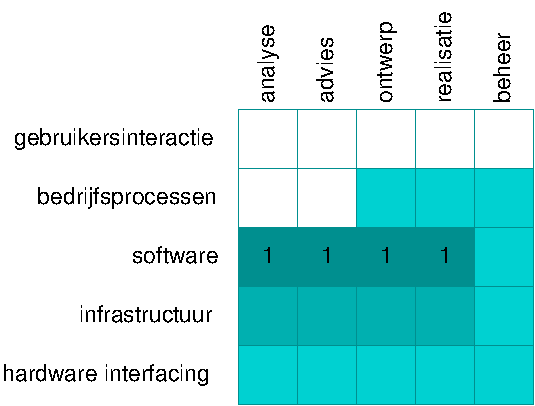
\includegraphics[width=7cm]{comptabel.pdf}
	\end{center}\\
	\hline
	\textbf{Learning objectives:} &
		At the end of the course, the student can:
			\begin{itemize}
               \item \textbf{use} and \textbf{design} recursive functions \texttt{FUNREC}
               \item \textbf{understand} the concept of abstraction through class definition \texttt{CLSABS}
               \item \textbf{use} and \textbf{design} classes without inheritance or interfaces \texttt{CLSDEF}
               \item \textbf{use} recursively defined lists \texttt{LISTS}
               \item \texttt{RECDATA}
               \item \textbf{use} standard predefined collections \texttt{STDDS}
			\end{itemize} \\
		
	\hline
\end{tabularx}
\newpage

\begin{tabularx}{\textwidth}{|>{\columncolor{lichtGrijs}} p{.26\textwidth}|X|}
	\hline
	\textbf{Content:}&
	\begin{itemize}
		\item basic concepts of data structures
		\item list: design of a well-known data structure
		\item functions as abstraction of instructions 
		\item Higher order functions and relation SQL (Python 3)
		\item methods within container of classes (Python 3)
		\item collection libraries: list, tuple, map, set (Python 3)
	\end{itemize} \\
	\hline
	\textbf{Course owners:} & \author\\
	\hline
	\textbf{Date:} & \today \\
	\hline
\end{tabularx}
\newpage

\newpage
\section{General description}
		Programming is one of the most ubiquitous activities within the field of ICT. Many business needs are centered around the gathering, elaboration, simulation, etc. of data through programs. \\
		
		This course covers intermediate aspects of building abstractions (functions, data structures, and classes) in the Python programming language (version 3). \\

	\subsection{Relationship with other teaching units}
		Subsequent programming courses build upon the knowledge learned during this course.	\\
		
		The course also provides a semantic background in order to understand the implementation of SQL queries within the framework of higher order (list) functions.	\\
		
		Knowledge acquired through the programming courses is also useful for the projects. A word of warning though: projects and development courses are largely independent, so some things that a student learns during the development courses are not used in the projects, some things that a student learns during the development courses are indeed used in the projects, but some things done in the projects are learned within the context of the project and not within the development courses.

\newpage
\section{Course program}
	The course is structured into six lectures. The six lectures take place during the six weeks of the course, but are not necessarily in a one-to-one correspondance with the course weeks. For example, lectures one and two are fairly short and can take place during a single week.

	\subsection{Lecture 1 - data structures}
		The first lecture covers ...

		\paragraph*{Topics}
			\begin{itemize}
				\item Mechanism of abstraction;
				\item The necessity for data structures;
				\item Data structures in Python (class);
				\item Semantics (Heap, Stack);
				\item Layers of abstraction.
			\end{itemize}

		\paragraph*{Activities}
			\begin{itemize}
				\item Let students follow instructions;
				\item Introduce elements of state and let students follow instructions with state (\textit{take N/4 steps forward; N is your age});
				\item Introduce elements of writable state and let students follow instructions with writable state (\textit{take N/4 steps forward; N is written under the yellow sticker});
				\item Introduce elements of decision-making and let students follow instructions with state and decision making (\textit{if the sun is shining, then take N/4 steps forward; otherwise, go sit down});
				\item Introduce elements of iteration and let students follow instructions with state, decision making, and iteration (\textit{divide the students in teams, and let run some script battling for the toy farm}).
			\end{itemize}

			\subsection{Lecture 2 - lists}
				The second lecture covers ...

				\paragraph*{Topics}
					\begin{itemize}
						\item The need for a variable to contain an \textit{unknown} number of values;
						\item Abstraction of list: \texttt{Node (Head), Tail, Empty};
						\item Implementation of list (Python 3);
						\item Semantics of list: \texttt{Heap and Stack}
					\end{itemize}

				\paragraph*{Activities}
					\begin{itemize}
						\item ...
					\end{itemize}


			\subsection{Lecture 3 - functions}
				The third lecture covers ...

				\paragraph*{Topics}
					\begin{itemize}
						\item Abstraction operations (functions)
						\item The need for functions;
						\item Creating and using functions in Python;
						\item Formal and actual parameters and return;
						\item Brief introduction to: scope (local and global variables) and visibility;
						\item Syntax and semantics;
						\item Introduction to recursion;
					\end{itemize}

			\subsection{Lecture 4 - higher order functions and SQL}
				The fourth lecture covers ...

				\paragraph*{Topics}
					\begin{itemize}
						\item What are higher order functions (HOF's) and \textit{why we do need them}?
						\item Functions as parameter;
						\item Lambda: $\lambda$-expressions (syntax and semantics);
						\item Fundamental operations on list: \texttt{transform, filter, fold};
						\item Using HOF's;
						\item SQL vs list HOF's.
					\end{itemize}

				\paragraph*{Activities}
					Call upon students to solve small riddles related to sample Python scripts on:

					\begin{itemize}
						\item Integers, strings, floats, bools;
						\item Integer, string, float, and bool varialbes;
						\item Semantics and post-conditions on variable-assignments.
						\item Integers, strings, floats, bool expressions;
						\item Conditional expressions;
						\item Semantics and post-conditions on expressions and conditional expressions.
					\end{itemize}

			\subsection{Lecture 5 - methods}
				The fifth lecture covers ...

				\paragraph*{Topics}
					\begin{itemize}
						\item Joining functions (methods) and data to classes;
						\item Designing a class;
						\item Concrete implementation of a class;
						\item Syntax and semantics;
						\item special method names;
						\item rebuilding the list data structure;
						\item Brief introduction immutability and mutability.
					\end{itemize}

				\paragraph*{Activities}
					Call upon students to solve small riddles related to sample Python scripts on:

					\begin{itemize}
						\item \texttt{if-then} and \texttt{if-then-else} statements;
						\item how many possible final states of a program;
						\item semantics and post-conditions on conditional statements.
					\end{itemize}


			\subsection{Lecture 6 - collections library}
				The sixth (and last) lecture covers ...

				\paragraph*{Topics}
					\begin{itemize}
						\item repeated behaviors;
						\item \texttt{while} statements;
						\item (slightly informal) semantics;
						\item (more than) exponential explosion of potential control-paths;
						\item expressive power of \texttt{while};
						\item \texttt{for} statements;
						\item (slightly informal) semantics;
						\item \texttt{for} as a \textit{limited} form of \texttt{while}.
					\end{itemize}

				\paragraph*{Activities}
					Call upon students to solve small riddles related to sample Python scripts on:

					\begin{itemize}
						\item \texttt{while} and \texttt{for} loops;
						\item how many possible final states of a program;
						\item semantics and post-conditions on loops.
					\end{itemize}

\newpage
\section{Assessment}
The course is tested with two exams: a series of practical assignments, a brief oral check of the practical assignments, and a theoretical exam. The final grade is determined as follows: \\

\texttt{if theoryGrade $\geq$ 75\% \& practicumCheckOK then return practicumGrade else return insufficient}

This means that the theoretical knowledge is a strict requirement in order to get the actual grade from the practicums, but it does not reflect your level of skill and as such does not further influence your grade.

\paragraph*{Motivation for grade}
A professional software developer is required to be able to program code which is, at the very least, \textit{correct}.

In order to produce correct code, we expect students to show:
\begin{inparaenum}[\itshape i\upshape)]
\item a foundation of knowledge about how a programming language actually works in connection with a simplified concrete model of a computer;
\item fluency when actually writing the code.
\end{inparaenum}

The quality of the programmer is ultimately determined by his actual code-writing skills, therefore the final grade comes only from the practicums. The quick oral check ensures that each student is able to show that his work is his own and that he has adequate understanding of its mechanisms. The theoretical exam tests that the required foundation of knowledge is also present to avoid away of programming that is exclusively based on intuition, but which is also grounded in concrete and precise knowledge about what each instruction does.


\subsection{Theoretical examination \modulecode}
The general shape of a theoretical exam for \texttt{\modulecode} is made up of a series of highly structured open questions. In each exam the content of the questions will change, but the structure of the questions will remain the same. For the structure (and an example) of the theoretical exam, see the appendix.


\subsection{Practical examination \modulecode}
Each week there is a mandatory assignment. The assignments of week 4, 5 and 6 will be graded. Each assignment is due the following week. The sum of the grades will be the $practicumGrade$. 
If the course is over and $practicumGrade$ is lower than $5,5$ then you can retry (herkansing) the practicum with one assignment which will test all learning goals and will replace the whole $practicumGrade$.
The following rules apply to the assignment:
\begin{itemize}
  \item The assignments are to be uploaded to N@tschool in the required space (Inlevermap);
  \item Only basic operations are allowed for the assignment unless explicit permitted otherwise; 
\end{itemize}
The oral check  (preferred during the practicums) is done on work uploaded to N@tschool:
\begin{itemize}
  \item two (2) questions per assignment about \textit{What does this line (these lines) do?}
  \item the exercise runs correctly
\end{itemize}


\subsection{Oral check \modulecode}
During the oral check, the teacher will verify ownership and competence with the code that was handed in during the practicum. This effectively determines the grade of the practicum. The procedure works as follows:

\begin{enumerate}
\item For each practicum, the teacher will \textbf{delete} some lines of code;
\item The student will then rewrite them from skratch;
\item Succesful restoring of the functionality will give the points for that assignment; failure in restoring the functionality will result in zero points for that practicum, independently of what was originally handed in.
\end{enumerate}

\newpage
\section*{Theoretical examination \modulecode}
The general shape of a theoretical exam for \texttt{DEV II} is made up of a series of highly structured open questions.


\paragraph{Question I: abstracting patterns with functions} \ \\

\textbf{General shape of the question:} \textit{Given a problem description, define one or more functions in order to solve the original problem.}

\ \\ 

\textbf{Concrete example of question:} \textit{Define a recursive \texttt{range} function to create a custom list (only use \texttt{Empty} and \texttt{Node}, see Appendix) with all the elements between two given numbers.}

\ \\ 

\textbf{Concrete example of answer:} \textit{The resulting code is:}

\begin{lstlisting}
def range(l, u):
  if l > u:
    return Empty()
  else:
    return Node(l, range(l+1,u))
\end{lstlisting}

\ \\ 

\textbf{Points:} \textit{25\%.}

\ \\ 

\textbf{Grading:} \textit{All points for correct function, minor mistakes (wrong check, some elements might be missing, etc.) half points, wrong function (infinite recursion, iterative version, etc.) zero points.}

\ \\ 

\textbf{Associated learning goals:} \texttt{FUNABS}, \texttt{FUNDEF}, \texttt{FUNREC}, \texttt{RECDATA}.

\ \\ 

\paragraph{Question II: runtime behaviour of functions} \ \\

\textbf{General shape of the question:} \textit{Given a function definition and a sample call, show stack and heap at all steps of the computation.}

\ \\ 

\textbf{Concrete example of question:} \textit{Given the following function definition and a sample call, show stack and heap at all steps of the computation.}
\lstset{
numbers=left
}
\begin{lstlisting}
def f(n):
  if n <= 1:
    return n
  else:
    return n * f(n-1)

f(3)
\end{lstlisting}
\lstset{
numbers=none
}
\ \\ 

\textbf{Concrete example of answer:} \textit{The last call of the stack is :}

\begin{lstlisting}
S: PC   f   PC   n   f   PC   n   f   PC   n
    7  nil   2   3  nil   2   2  nil   2   1
H: always empty
\end{lstlisting}

\textit{The stack will then unwind as follows:}

\begin{lstlisting}
S: PC   f   PC   n   f   PC   n   f   PC   n
    7  nil   2   3  nil   2   2   1   3   1
\end{lstlisting}

\ \\

\begin{lstlisting}
S: PC   f   PC   n   f   PC   n
    7  nil   2   3  2*1   4   2
\end{lstlisting}

\ \\

\begin{lstlisting}
S: PC   f   PC   n
    7  3*2   4   3
\end{lstlisting}

\ \\ 

\textbf{Points:} \textit{25\%.}

\ \\ 

\textbf{Grading:} \textit{All points for all stack frames and values, half points for at least half correct stack frames and values, otherwise zero points.}

\ \\ 

\textbf{Associated learning goals:} \texttt{FUNABS}, \texttt{FUNDEF}, \texttt{FUNREC}, \texttt{RECDATA}.

\ \\ 

\paragraph{Question III: classes} \ \\

\textbf{General shape of the question:} \textit{Given a description, give the implementation of a class and its methods in Python.}

\ \\ 

\textbf{Concrete example of question:} \textit{Define a \texttt{Counter} class with a single method, \texttt{Tick}, which increments the internal \texttt{cnt} of the class. Also provide an implementation of \texttt{\_\_str\_\_)}}

\ \\ 

\textbf{Concrete example of answer:} \textit{The resulting code is:}

\begin{lstlisting}
class Counter:
  def __init__(self):
    self.cnt = 0
  def Tick(self):
    self.cnt = self.cnt + 1
  def __str__(self):
    return "Ticked " + str(self.cnt) + " times"
\end{lstlisting}

\ \\ 

\textbf{Points:} \textit{25\%.}


\textbf{Grading:} \textit{All points for correct answer, half points for at least correct implementation of methods \_\_init\_\_ and Tick, otherwise zero points.}

\ \\ 

\textbf{Associated learning goals:} \texttt{CLSABS}, \texttt{CLSDEF}.

\ \\

\paragraph{Question IV: standard libraries} \ \\

\textbf{General shape of the question:} \textit{Define a loop that performs some simple operation on a standard data structure.}

\ \\ 

\textbf{Concrete example of question:} \textit{Define a loop that sums all positive elements of a Python list \texttt{l} which contains only integers. Finally, print the sum.}

\ \\ 

\textbf{Concrete example of answer:} \textit{The resulting code is:}

\begin{lstlisting}
sum = 0
for x in l:
  if x > 0:
    sum = sum + x
print(sum)
\end{lstlisting}

\ \\ 

\textbf{Points:} \textit{25\%.}

\ \\ 

\textbf{Grading:} \textit{All points for correct answer, otherwise zero points.}

\ \\ 

\textbf{Associated learning goals:} \texttt{ARR}.

\ \\

\newpage
\section*{Exam sample}
What follows is a concrete example of the exam.


\paragraph{Question I: abstracting patterns with functions} \ \\

\textit{Define a \texttt{map} function to transform all elements of the input list (defined with \texttt{Empty} and \texttt{Node}, see Appendix) according to a given function \texttt{f}.}

\ \\ 

\textbf{Answer:} \textit{The resulting code is:}

\begin{lstlisting}
def map(l,f):
  if l.IsEmpty():
    return Empty()
  else:
    return Node(f(l.Head()), map(l.Tail(), f))
\end{lstlisting}

\ \\ 

\textbf{Points:} \textit{25\%.}

\ \\ 

\textbf{Grading:} \textit{All points for correct function, minor mistakes (wrong check, some elements might be missing, etc.) half points, wrong function (infinite recursion, iterative version, etc.) zero points.}

\ \\ 

\paragraph{Question II: runtime behaviour of functions} \ \\

\textit{Given the following function definition and a sample call, show stack and heap at all steps of the computation.}

\begin{lstlisting}
def filter(l,p):
  if p(l.head):
    return Node(l.head, filter(l.tail, p))
  else:
    return filter(l.tail, p)

filter(Node(1,Node(2,Empty())), lambda x: x >= 2)
\end{lstlisting}

\ \\ 

\textbf{Answer:} \textit{Each call of the stack should contain a value for \texttt{l} and one for \texttt{p}. The heap should contain a value for each node of the list, and for the lambda function of \texttt{p}.}

\begin{lstlisting}
S: PC   filter   PC     l       p
    7    nil      2   ref(2)  ref(3)
    
H: 0             1                        2                      3
  [ ]   [head->1;tail->ref(0)]   [head->2;tail->ref(1)]   lambda x: x >= 2
\end{lstlisting}

\textit{After each step, the stack grows but the heap does not:}

\begin{lstlisting}
S: PC   filter   PC     l       p    filter   PC     l       p
    7    nil      5   ref(2)  ref(3)  nil      2   ref(1)  ref(3)
    
H: 0             1                        2                      3
  [ ]   [head->1;tail->ref(0)]   [head->2;tail->ref(1)]   lambda x: x >= 2
\end{lstlisting}

The rest follows similarly. Watch out for reconstruction of recursive result with correct elements wrt returned value of \texttt{p(l.head)}.

\textbf{Points:} \textit{25\%.}

\ \\ 

\textbf{Grading:} \textit{All points for all stack frames and values, half points for at least half correct stack frames and values, otherwise zero points.}

\ \\ 

\paragraph{Question III: classes} \ \\

\textbf{Concrete example of question:} \textit{Define a \texttt{Train} class with attributes:
\begin{itemize}
\item \texttt{Position} of the ship in the map (a 2D vector, see Appendix)
\item amount of \texttt{Passengers}
\item amount of \texttt{Containers}
\end{itemize}
and methods:
\begin{itemize}
\item \texttt{TravelTo} that receives a \texttt{Station}\footnote{The \texttt{Station} class has at least the attributes \texttt{Position}, \texttt{WaitingPassengers}, \texttt{WaitingContainers}} as a destination and changes
\begin{itemize}
\item the \texttt{Position} of the train to the \texttt{Position} of the station
\item the \texttt{Passengers} of the train (and the \texttt{WaitingPassengers} of the station)
\item the \texttt{Containers} of the train (and the \texttt{WaitingContainers} of the station)
\end{itemize}
\end{itemize}}

\ \\ 

\textbf{Points:} \textit{25\%.}

\ \\ 

\textbf{Grading:} \textit{All points for all attributes and methods, half points for at least half correct attributes and methods, otherwise zero points.}

\ \\ 

\textbf{Answer:} \textit{The implemented class is:}

\begin{lstlisting}
class Station:
  def __init__(self, p, wp, wc):
    self.Position = p
    self.WaitingPassengers = wp
    self.WaitingContainers = wc

class Ship:
  def __init__(self, p):
    self.Position = p
    self.Passengers = 0
    self.Containers = 0
  def NavigateTo(self, port):
    self.Position = port.Position
    self.Passengers = port.WaitingPassengers
    port.WaitingPassengers = 0
    self.Containers = port.WaitingContainers
    port.WaitingContainers = 0
\end{lstlisting}

\paragraph{Question IV: standard libraries} \ \\

\textbf{Concrete example of question:} \textit{Define a loop that adds all odd elements in a given Python list \texttt{l} which contains only integers. If the list is empty the result should be \texttt{0}. Finally, print the result.}

\ \\ 

\textbf{Points:} \textit{25\%.}

\ \\ 

\textbf{Grading:} \textit{All points for correct iteration and sum, half points for wrong use of indices or wrong iteration, zero points otherwise.}

\ \\ 

\textbf{Answer:} \textit{The implemented class is:}

\begin{lstlisting}
l = [1,2,3,4]
res = 0
for x in l:
  if x % 2 == 1:
    res = res + x
print(res)
\end{lstlisting}

\subsection{Exam appendix}

\paragraph{List implementation}
\begin{lstlisting}
class Empty:
  def IsEmpty(): return True
Empty = Empty()

class Node:
  def IsEmpty(): return False
  def Head(self): return self.Head
  def Tail(self): return self.Tail
  def __init__(self, x, xs):
    self.head = x
    self.tail = xs
\end{lstlisting}

\paragraph{Vector2 implementation}
\begin{lstlisting}
class Vector2:
  def __init__(self, x, y):
    self.X = x
    self.Y = y
  def Length(self):
    return math.sqrt(self.X * self.X + self.Y * self.Y)
  def __neg__(self):
    return Vector2(-self.X, -self.Y)
  def __add__(self, other):
    return Vector2(self.X + other.X, self.Y + other.Y)
  def __sub__(self, other):
    return self + (-other);
  def __mul__(self, k):
    return Vector2(self.X * k, self.Y * k)
  def __str__(self):
    return "(" + str(self.X) + "," + str(self.Y) + ")"
  def Zero(): 
    return Vector2(0.0, 0.0)
  def UnitX(): 
    return Vector2(1.0, 0.0)
  def UnitY(): 
    return Vector2(0.0, 1.0)
\end{lstlisting}

%##############################

\newpage
%\bibliographystyle{plain}
%\bibliography{references}
%\newpage
\section*{Bijlage 1: Toetsmatrijs}
	\begin{tabular}{|p{1cm}|p{4cm}|}
		\hline
		Learning goals & Dublin descriptors \\
		\hline
		\texttt{LMC} & 1, 4 \\
		\hline
		\texttt{CMC} & 1, 4 \\
		\hline
		\texttt{VAR} & 1, 2, 4 \\
		\hline
		\texttt{EXPR} & 1, 2, 4 \\
		\hline
		\texttt{COND} & 1, 2, 4 \\
		\hline
		\texttt{LOOP} & 1, 2, 4 \\
		\hline
	\end{tabular}
	
	\vspace{1cm}

	Dublin-descriptors:
	\begin{enumerate}
		\item Knowledge and understanding
		\item Applying knowledge and understanding
		\item Making judgments
		\item Communication
		\item Learning skills
	\end{enumerate}

%\newpage
%\section*{Bijlage 2: Voorbeeldtoets}

		Dit hoofdstuk bevat de beschrijving van de procedures om voor beoordeling in aanmerking te komen.\\
		Bijvoorbeeld voldoende aanwezigheid, 80\% van de opdrachten hebben ingeleverd, presentaties hebben verricht etc.\\

		Verder wordt zo gedetailleerd mogelijk beschreven hoe er tot een cijfer wordt gekomen en welke rollen er door docenten en ander betrokkenen hierbij vervuld worden. \\

		Geef een verantwoording van de toets; wat wordt getoetst, waarom is voor deze vorm gekozen.\\

		Vul een toetsmatrijs in voor de toets (zie bijlage).\\

		Beschrijf ook duidelijk de \textbf{herkansingsmogelijkheden}. \\

		Neem in geval van een schriftelijk tentamen een voorbeeldtoets op als bijlage.\\
		Geef daarbij per deelvraag het aantal te verdienen punten aan. \\

		Bij een schriftelijk rapport. Geef de beoordelingscriteria aan met daarbij de mogelijke score en de onderlinge weging. \\

		Toetsduur: \\

		Hoe en wanneer krijgt de student feedback?\\
%\newpage
%\section*{Bijlage 3: Studielast normering in ects}

		Dit hoofdstuk bevat de beschrijving van de procedures om voor beoordeling in aanmerking te komen.\\
		Bijvoorbeeld voldoende aanwezigheid, 80\% van de opdrachten hebben ingeleverd, presentaties hebben verricht etc.\\

		Verder wordt zo gedetailleerd mogelijk beschreven hoe er tot een cijfer wordt gekomen en welke rollen er door docenten en ander betrokkenen hierbij vervuld worden. \\

		Geef een verantwoording van de toets; wat wordt getoetst, waarom is voor deze vorm gekozen.\\

		Vul een toetsmatrijs in voor de toets (zie bijlage).\\

		Beschrijf ook duidelijk de \textbf{herkansingsmogelijkheden}. \\

		Neem in geval van een schriftelijk tentamen een voorbeeldtoets op als bijlage.\\
		Geef daarbij per deelvraag het aantal te verdienen punten aan. \\

		Bij een schriftelijk rapport. Geef de beoordelingscriteria aan met daarbij de mogelijke score en de onderlinge weging. \\

		Toetsduur: \\

		Hoe en wanneer krijgt de student feedback?\\
\printindex


\end{document}
